\newpage
\section{Homoskedasticity and Heteroskedasticity}
Intro intro baseret på...

In this section we wish to introduce \homo and \hetero, in order to determine if our model considers all important factors affecting our data. If our model is precise the variance of the error term should be consistent for all the explanatory variables in the model and thus do not depend on the explanatory variables. First we define what \homo and \hetero is. 

\begin{definition}[Homoskedasticity and heteroskedasticity]
When the variance of the error term does not depend on the explanatory variables $\textbf{X}$ the errors is said to be \homo, thus the errors should obey

\begin{align*}
    \var(\epsilon | \textbf{X}) = \var(\epsilon) = \sigma^2
\end{align*}

If this is not satisfied the error is said to be \hetero. 

\end{definition}

The intuition behind \homo is that the variance of the error does not depend on the explanatory variables $X$, hence it does not change for any value given to the explanatory variables. Conversely if the variance of the error term changes with any of the explanatory variables the error term is \hetero. The greater the error term changes the greater a violation of \homo is it. 


Homoskedasticity and \hetero can be illustrated as in figure \ref{fig:homo_with_dependent_up_axis} and \ref{fig:hetero_with_dependent_up_axis}. 




----------------------------------


\begin{figure}[h]
\centering
\begin{subfigure}[b]{0.4\textwidth}
    \centering
    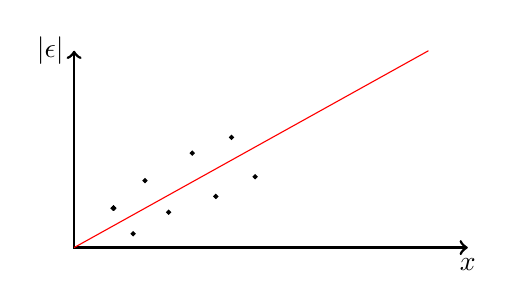
\begin{tikzpicture}[scale=0.5]
            \draw[<->,line width=1] (10,0)node[below]{$x$}--(0,0)--(0,5)node[left]{$|\epsilon|$};
            \draw[red] plot [left] coordinates {(0,0) (9,5)};
            \filldraw (1,1) circle (0.5mm);
            \filldraw (1.5,0.35) circle (0.5mm);
            \filldraw (1.8,1.7) circle (0.5mm);
            \filldraw (2.4,0.9) circle (0.5mm);
            \filldraw (3,2.4) circle (0.5mm);
            \filldraw (3.6,1.3) circle (0.5mm);
            \filldraw (4,2.8) circle (0.5mm);
            \filldraw (4.6,1.8) circle (0.5mm);
            \filldraw (1,1) circle (0.5mm);
            \filldraw (1,1) circle (0.5mm);
            \filldraw (1,1) circle (0.5mm);
            \filldraw (1,1) circle (0.5mm);
            \filldraw (1,1) circle (0.5mm);
            \filldraw (1,1) circle (0.5mm);
            \filldraw (1,1) circle (0.5mm);
            \filldraw (1,1) circle (0.5mm);
        \end{tikzpicture}
    \caption{JEG RETTER DEN HOMO med afhængig}
    \label{fig:homo_with_dependent_up_axis}
\end{subfigure}%
~
\begin{subfigure}[b]{0.4\textwidth}
\centering
    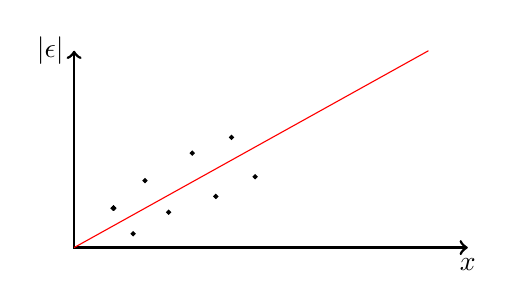
\begin{tikzpicture}[scale=0.5]
            \draw[<->,line width=1] (10,0)node[below]{$x$}--(0,0)--(0,5)node[left]{$|\epsilon|$};
            \draw[red] plot [left] coordinates {(0,0) (9,5)};
            \filldraw (1,1) circle (0.5mm);
            \filldraw (1.5,0.35) circle (0.5mm);
            \filldraw (1.8,1.7) circle (0.5mm);
            \filldraw (2.4,0.9) circle (0.5mm);
            \filldraw (3,2.4) circle (0.5mm);
            \filldraw (3.6,1.3) circle (0.5mm);
            \filldraw (4,2.8) circle (0.5mm);
            \filldraw (4.6,1.8) circle (0.5mm);
            \filldraw (1,1) circle (0.5mm);
            \filldraw (1,1) circle (0.5mm);
            \filldraw (1,1) circle (0.5mm);
            \filldraw (1,1) circle (0.5mm);
            \filldraw (1,1) circle (0.5mm);
            \filldraw (1,1) circle (0.5mm);
            \filldraw (1,1) circle (0.5mm);
            \filldraw (1,1) circle (0.5mm);
        \end{tikzpicture}
    \caption{JEG RETTER DEN HETERO med afhængig}
    \label{fig:hetero_with_dependent_up_axis}
\end{subfigure}
\end{figure}

---------------------------------

In the case of \homo the variance is consistent for all values of $\textbf{X}$, to which the standard errors do not depend on the explanatory variables. In the case of \hetero the variance increases as $\textbf{X}$ increases. An example of this can be if you consider family income and spending on luxury items. if the income is low most will be spend on necessity items such as food, if the income increases is the possibility but not the necessity of spending more on luxury items, thus there will be a greater variance in the consumption of luxury goods. In short \hetero arises when variances of unobserved factors changes over different segments in the sample space. 



\subsection{Problems with \hetero}


-----------------
MANGLER UDLED MANGLER f-test og t-test I FOIRHOLD TIL OLS LIGNINGER
- .-----------------


Heteroskedasticity is a problem within OLS because OLS assumes all error terms origin from a sample space with constant variance, which is \homo. Estimators will no longer be the \textbf{best linear unbiased estimator (BLUE)}. This is beacuse the OLS no longer will give the estimate with the smallest variance for the unbiased estimators. OLS gives equal weight to all observation and in the case of \hetero observations with greater variance have greater impact but less information and vice versa. Heteroskedasticity therefor makes the estimations less precise. This if the variance of the error term is not constant \textit{t statistics} and \textit{confidence intervals} will be invalid no matter the sample size, because the regression coefficients are estimated wrongly.

-----------

Remember our linear regression




























\subsection{test for \hetero}






